\hypertarget{_simple_neural_creator_8cpp}{
\section{/Users/mcasl/pc-\/ule/Trabajo/investigacion/AMORE/AMORE-\/WC/AMORE-\/WC/pkg/AMORE/src/SimpleNeuralCreator.cpp File Reference}
\label{_simple_neural_creator_8cpp}\index{/Users/mcasl/pc-\/ule/Trabajo/investigacion/AMORE/AMORE-\/WC/AMORE-\/WC/pkg/AMORE/src/SimpleNeuralCreator.cpp@{/Users/mcasl/pc-\/ule/Trabajo/investigacion/AMORE/AMORE-\/WC/AMORE-\/WC/pkg/AMORE/src/SimpleNeuralCreator.cpp}}
}
{\ttfamily \#include \char`\"{}package.h\char`\"{}}\par
{\ttfamily \#include \char`\"{}classHeaders/Container.h\char`\"{}}\par
{\ttfamily \#include \char`\"{}classHeaders/Neuron.h\char`\"{}}\par
{\ttfamily \#include \char`\"{}classHeaders/NeuralCreator.h\char`\"{}}\par
{\ttfamily \#include \char`\"{}classHeaders/NeuralFactory.h\char`\"{}}\par
{\ttfamily \#include \char`\"{}classHeaders/NeuralNetwork.h\char`\"{}}\par
{\ttfamily \#include \char`\"{}classHeaders/SimpleNeuralCreator.h\char`\"{}}\par
Include dependency graph for SimpleNeuralCreator.cpp:
\nopagebreak
\begin{figure}[H]
\begin{center}
\leavevmode
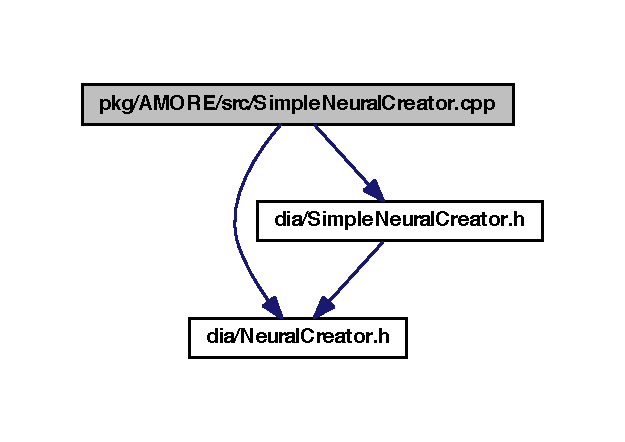
\includegraphics[width=400pt]{_simple_neural_creator_8cpp__incl}
\end{center}
\end{figure}
This graph shows which files directly or indirectly include this file:
\nopagebreak
\begin{figure}[H]
\begin{center}
\leavevmode
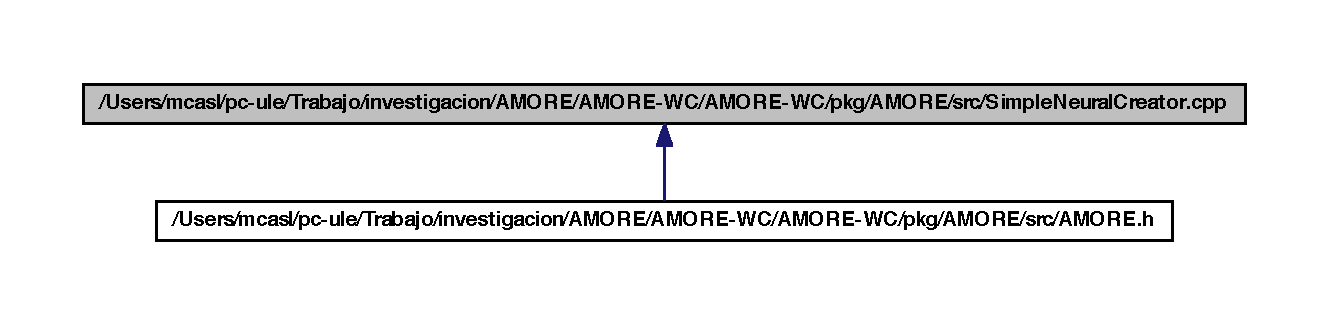
\includegraphics[width=400pt]{_simple_neural_creator_8cpp__dep__incl}
\end{center}
\end{figure}
